\documentclass[aspectratio=1610]{beamer}
\setbeamersize{text margin left=7mm,text margin right=5mm}
\usefonttheme[onlymath]{serif}
\usetheme{default}
\usefonttheme{professionalfonts}
%\setbeamertemplate{navigation symbols}{} 
\beamertemplatenavigationsymbolsempty
\addtobeamertemplate{navigation symbols}{}{
    \usebeamerfont{footline}
    \usebeamercolor[fg]{footline}
    %\hspace{1em}
    \footnotesize\insertframenumber\,%/\inserttotalframenumber
}

% cSpell:disable
\definecolor{rcomment}{rgb}{0.3, 0.3, 0.3}  % darkgrey
\definecolor{rred}{rgb}{0.7,0.2,0.2}        % red
\definecolor{rblue}{rgb}{0.2,0.2,0.7}       % blue (blended blue of beamer)
\definecolor{rpurple}{rgb}{0.45, 0.0, 0.9}  % violett
\definecolor{rpink}{rgb}{0.8, 0.0, 0.4}     % pink
\definecolor{rgreen}{rgb}{0.1, 0.5, 0.1}    % darkgreen
\definecolor{rorange}{rgb}{0.8, 0.4,0}      % orange
\definecolor{rblack}{rgb}{0, 0, 0}          % black
\definecolor{deeptuerkis}{rgb}{0, 0.5, 0.5} % Türkis
\definecolor{darkgreen}{rgb}{0,0.5,0}
\definecolor{blendedblue}{rgb}{0.2,0.2,0.7}
\newcommand{\important}[1]{{\color{green!60!black}#1}}

% \documentclass{beamer}
% \mode<presentation> {
%   \usetheme{Singapore}
%   \setbeamertemplate{navigation symbols}{}
%   \setbeamertemplate{footline}[frame number]
% }

\usepackage[utf8]{inputenc}
\usepackage{caption}
\usepackage{nicefrac}
\usepackage{varwidth}
\usepackage{amsmath}
\usepackage{hyperref}
\usepackage{color}
\usepackage{xcolor}
\usepackage[linesnumbered, ruled, noend]{algorithm2e}
\usepackage{appendixnumberbeamer}
\usepackage{booktabs}
\usepackage{multirow}
\usepackage{multimedia}


\usepackage{natbib}
% \usepackage[backend=bibtex,style=authoryear-comp]{biblatex}
% \bibliography{bibliography}

\usepackage[draft,nomargin,inline]{fixme}  % add final for disabling remarks
\fxsetface{inline}{\itshape}
\fxsetface{env}{\itshape}
%\fxuselayouts{margin}
%\fxuselayouts{inline}
\fxusetheme{color}

\usepackage{tikz}
\usepackage{pgfplots}
\usetikzlibrary{calc, decorations.markings}
\tikzset{vertex/.style={circle, draw=black}}
\tikzset{tr/.style={draw=white, fill=white, sloped}}
\tikzset{del/.style={draw=red, text=red}}
\tikzset{layer/.style={rectangle, draw=black, minimum width=1.5cm, minimum height=0.75cm}}
\tikzset{plus/.style={
  circle, draw=black, minimum width=0.3cm, inner sep=0cm, outer sep=0cm,
  path picture={
    \draw[black] (path picture bounding box.south) -- (path picture bounding box.north)
                 (path picture bounding box.west) -- (path picture bounding box.east);
  }
}}
\tikzset{buswidth/.style={decoration={
  markings,
  mark=at position 0.5 with {\node[font=\footnotesize] {/};\node[below=3pt] {\tiny #1};}
}, postaction={decorate}}}

\pgfplotsset{compat=1.18}


\newcommand{\tmax}{\ensuremath{t^\mathrm{max}}}
\newcommand{\plim}{\ensuremath{p^\mathrm{lim}}}
\newcommand{\ILP}{\ensuremath{\mathrm{ILP}}}
\newcommand{\ppath}{\ensuremath{p^\mathrm{path}}}
\newcommand{\Tavail}{T^\mathrm{avail}}
\newcommand{\Irej}{I^\mathrm{rej}}
\newcommand{\Greedy}{\textsc{Greedy}}
\newcommand{\Markov}{\textsc{Markov}}

% \renewcommand{\thefootnote}{\fnsymbol{footnote}}
% cSpell:enable

\title{Generative AI for Combinatorial Optimization:\\
Some Personal Experiences}

\author{Günther R.\ Raidl}
\date{Workshop on AI for Optimisation and Decision Making 2026\\ Victoria University of Wellington, NZ\\February 24, 2026}
\titlegraphic{\includegraphics[height=7mm]{graphics/logo-tuwien-informatics.png}\quad
	\includegraphics[height=7mm]{graphics/AClongColor.pdf}}

\institute[]{\normalsize Algorithms and Complexity Group, TU Wien, Austria,\\
    \texttt{raidl@ac.tuwien.ac.at}\\[1ex]
}

\logo{\includegraphics[height=15pt]{graphics/logo.pdf}\vspace{245pt}} % Logo on top right

% cSpell:disable
\definecolor{rred}{rgb}{0.7,0.2,0.2}         % red
\newcommand{\hl}[1]{\textcolor{rred}{#1}}    % highlight

\definecolor{rgreen}{rgb}{0.216,0.784,0.216} % green
\definecolor{rblue}{rgb}{0.216,0.443,0.784}  % blue
\definecolor{rorange}{rgb}{1.0,0.4,0.0}      % orange

\definecolor{orange}{RGB}{255,100,66}
\definecolor{seaborn0}{HTML}{1f77b4}
\definecolor{seaborn1}{HTML}{ff7f0e}
\definecolor{seaborn2}{HTML}{2ca02c}
\definecolor{seaborn3}{HTML}{d62728}
\definecolor{seaborn4}{HTML}{9467bd}
\definecolor{seaborn5}{HTML}{8c564b}
\definecolor{seaborn6}{HTML}{e377c2}
\definecolor{seaborn7}{HTML}{7f7f7f}
\definecolor{seaborn8}{HTML}{bcbd22}
\definecolor{seaborn9}{HTML}{17becf}

\newbool{printlegend}

\newcommand{\cumuldistr}[7]{ % Arguments: source directory, data series, width, height, x label, y label, title
  \begin{tikzpicture}
    \begin{semilogxaxis}[%
          width={#3},
          height={#4},
          title style={align=center},
          title={\large #7},
          xlabel style={at={(axis description cs:0.5,0.05)},anchor=north},
          xlabel=#5,
          ylabel style={align=center},
          ylabel=#6,
          every axis plot post/.append style={mark=none},
          every axis plot/.append style={thick},
          legend entries={GNN,Random,Sorted,Hooker},
          \ifbool{printlegend}{
            legend columns=1,
            legend pos=south east,
          }{
            legend to name=legend:cumuldistr-#1-#2,
            legend columns=-1,
          }
          ]
      \addplot+[seaborn0, solid]  table [x=#2, y=no_instances, col sep=comma, mark=none] {#1/pgdeletion_#2.csv};
      \addplot+[seaborn1, dashed] table [x=#2, y=no_instances, col sep=comma, mark=none] {#1/deletion_#2.csv};
      \addplot+[seaborn2, dashed] table [x=#2, y=no_instances, col sep=comma, mark=none] {#1/sdeletion_#2.csv};
      \addplot+[seaborn3, dashed] table [x=#2, y=no_instances, col sep=comma, mark=none] {#1/hdeletion_#2.csv};
    \end{semilogxaxis}
  \end{tikzpicture}
}
% cSpell:enable
\renewcommand{\footnotesize}{\scriptsize}

\begin{document}{}


\part{Main}

\begin{frame}
  \titlepage
\end{frame} 


\begin{frame}{Main Research Interests of G.~R.}


\medskip 
\begin{minipage}{0.45\textwidth}
  \begin{itemize}
      \item Combinatorial optimization (COP)
      \item Metaheuristics
      \item Mathematical programming
      \item Constraint programming
      \item Machine learning
      \item \important{\bf Hybrid approaches} incl.\ matheuristics, learning + classical algorithms for COP
  \end{itemize}
\end{minipage}\qquad
\begin{minipage}{0.4\textwidth}
    \structure{Application areas}
    \begin{itemize}
      \item Transport optimization
      \item Scheduling
      \item Network design
      \item Problems in bioinformatics
      \item Cutting and packing
    \end{itemize}
  \end{minipage}

  \bigskip
  \includegraphics[width=\textwidth]{graphics/AC-TU-Wien.jpg}
\end{frame}


% \begin{frame}{Selected Ongoing Projects}
% \begin{itemize}
%   \itemsep3.5ex
%   \item \structure{Dynamic Vehicle Routing Problems with Focus on E-mobility \& Learning}
%   \begin{itemize}
%     \item with T.~Rodemann et al., Honda Research Institute Europe
%     \item with Y. Mei, Victoria University of Wellington, NZ
%   \end{itemize}

%   \includegraphics[width=0.8\textwidth]{graphics/darp-bss-example.jpg}
% \end{itemize}
% \end{frame}


% \begin{frame}{Selected Ongoing Projects (contd.)}
% \begin{itemize}
% 	\itemsep3.5ex
% 	\item \structure{Cooperative Personnel Scheduling}
% 	\begin{itemize}
% 	\item with S.~Limmer et al., Honda Research Institute Europe
% 	\end{itemize}

% 	\includegraphics[width=0.6\textwidth]{graphics/coopsched.png}
% \end{itemize}
% \end{frame}
	
% \begin{frame}{Selected Ongoing Projects (contd.)}
% 	\begin{itemize}
% 	  \itemsep3.5ex
% 	  \item \structure{Roman Domination Problems, Influence Maximization Problems, and Variants}
% 	  \begin{itemize}
% 		\item with M. Djukanovic et al., Univ.\ of Banja Luka, Bosnia and Herzegovina
% 	  \end{itemize}

% 	  \bigskip
% 	  \includegraphics[width=0.7\textwidth]{graphics/influence_maximization.png}
% 	\end{itemize}
% \end{frame}
	
% \begin{frame}{Selected Ongoing Projects (contd.)}
% 	\begin{itemize}
% 	  \itemsep3.5ex
% 	  \item Doctoral College Vienna Graduate School on Computational Optimization
% 	  \begin{itemize}
% 		\item with University of Vienna, IST Austria, Vienna University of Economics and Business
% 	  \end{itemize}

% 	  \includegraphics[width=0.5\textwidth]{graphics/vgsco.png}
% 	\end{itemize}
% \end{frame}
	

% \begin{frame}{Recent Industry Colloaborations}
% \begin{itemize}
% \itemsep3.5ex
% 	\item \structure{Minimizing waste in cutting glass, wood, and steel}
% 	\begin{itemize}
% 	\item with Lodestar Inc., Eurosoft GmbH.
% 	\end{itemize} 

% 	\bigskip
% 	\includegraphics[width=0.34\textwidth, angle=90]{graphics/cutting_example.png}
% \end{itemize}  
% \end{frame}


% \begin{frame}{Recent Industry Colloaborations (contd.)}
% 	\begin{itemize}
% 	\itemsep3.5ex
% 		\item \structure{Public Bike Sharing Station Planning and Rebalancing}
% 		\begin{itemize}
% 		\item with City Bike Wien, NextBike, Austrian Institute of Technology
% 		\end{itemize} 
	
% 		\bigskip
% 		\includegraphics[width=0.8\textwidth]{graphics/BBSS.jpg}
% 	\end{itemize}  
% \end{frame}
	

% \begin{frame}{Recent Industry Colloaborations (contd.)}
% 	\begin{itemize}
% 	\itemsep3.5ex
% 		\item \structure{Planning Battery Exchange Stations for Electric Scooters}
% 		\begin{itemize}
% 		\item with Honda Japan, Honda Research Institute Europe
% 		\end{itemize} 
	
% 		\bigskip
% 		\includegraphics[width=0.6\textwidth]{graphics/bex.png}
% 	\end{itemize}  
% \end{frame}


% \begin{frame}{Recent Industry Colloaborations (contd.)}
% 	\begin{itemize}
% 	\itemsep3.5ex
% 		\item \structure{Transport Optimization for an Online Supermarket with Within-the-Hour Delivery}
% 		\begin{itemize}
% 		\item with Alfies GmbH
% 		\end{itemize} 
	
% 		\bigskip
% 		\includegraphics[width=0.6\textwidth]{graphics/alfies.jpg}
% 	\end{itemize}  
% \end{frame}
	
% --------------------------------------------------------

\begin{frame}{Outline}
	\begin{itemize}
		\itemsep4ex
		\item Few words on Large Language Models (LLMs) for Comb.~Opt.
		\item Generative Flow Networks (GFlowNets) for Comb.~Opt.
		\item Denoising Diffusion Models (DDMs) for Comb.~Opt.
		\item Conclusions and Outlook
	\end{itemize}
\end{frame}

% -------------------------------------------------

\begin{frame}[plain]
	\centering
	\vfill
	{\huge\structure{Large Language Models (LLMs)\\ for Combinatorial Optimization}}
	\vfill
\end{frame}

\begin{frame}{Large Language Models (LLMs) for Combinatorial Optimization}
	\begin{itemize}
		\itemsep4ex
		\item Directly throwing a LLM at a hard COP rarely works due to the structural complexities
		\pause
		\item Approaches where LLMs generate code for solving COPs 
		%\item Approaches where LLMs utilize existing solvers
	\end{itemize}
\end{frame}

\begin{frame}{FunSearch: Searching in the Function Space}

\vspace*{1ex}
\structure{\it Romera-Paredes, B. et al., 2024. Mathematical discoveries from program search with large language models. Nature 625, 468--475.}
\begin{center}
	\includegraphics[width=0.6\linewidth]{graphics/funsearch}

\end{center}
\begin{itemize}
	\item Evolutionary algorithm
	\item based on LLM paired with a systematic evaluator
	\item applied to cap set problem (in extremal combinatorics) and \movie[externalviewer]{online bin packing example}{graphics/binpack_animation.mp4} %https://storage.googleapis.com/gdm-deepmind-com-prod-public/media/media/binpack_animation_v3_DcLQBh5.mp4}
\end{itemize}
\end{frame}

\begin{frame}{Large Language Models (LLMs) and Combinatorial Optimization}
	\begin{itemize}
		\itemsep4ex
		\item Directly throwing a LLM at a hard COP rarely works due to the structural complexities
		\item Approaches where LLMs generate code for solving COPs 
		\item Using LLMs as front-end to dedicated solvers
	\end{itemize}
\end{frame}

\begin{frame}{Using LLMs as Front-End to Existing Solvers}

Example:

\bigskip
\begin{itemize}
	\itemsep2ex
	\item \important{Gurobi}: a state-of-the-art mixed integer linear programming (MILP) solver
	\item Modeling problems as MILPs is often considered an ``art''
	\item Let LLM translate a natural-language problem description into a MILP formulation
	\begin{itemize}
		\item Gurobot: Specialized LLM
		\item Gurobi AI Assistant
	\end{itemize}
	\item Gurobi MCP server: allows an LLM to actually \emph{use} Gurobi as backend
\end{itemize}

% cSpell:disable
\begin{center}
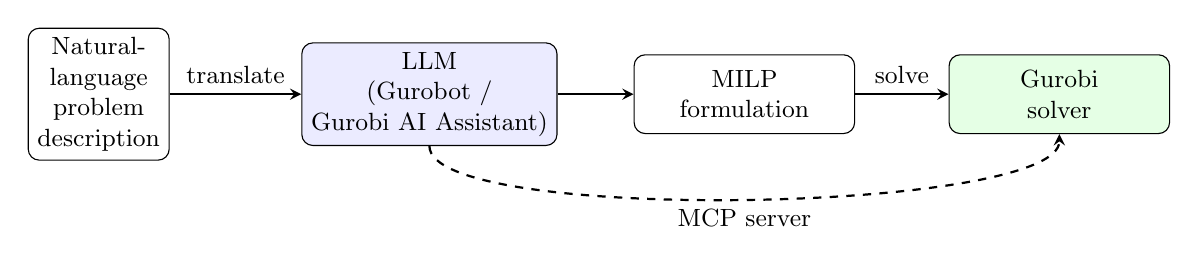
\begin{tikzpicture}[font=\small,>=stealth]
  % Nodes
  \node[draw, rounded corners, align=center, minimum width=1.6cm, minimum height=1.0cm] (nl) at (0,0)
    {Natural-\\language\\problem \\description};

  \node[draw, rounded corners, align=center, minimum width=2.8cm, minimum height=1.0cm, fill=blue!8] (llm) at (4.2,0)
    {LLM\\(Gurobot /\\Gurobi AI Assistant)};

  \node[draw, rounded corners, align=center, minimum width=2.8cm, minimum height=1.0cm] (milp) at (8.2,0)
    {MILP\\formulation};

  \node[draw, rounded corners, align=center, minimum width=2.8cm, minimum height=1.0cm, fill=green!10] (grb) at (12.2,0)
    {Gurobi\\solver};

  % Main flow
  \draw[->, thick] (nl) -- node[above] {translate} (llm);
  \draw[->, thick] (llm) -- (milp);
  \draw[->, thick] (milp) -- node[above] {solve} (grb);

  % MCP link
  \draw[->, thick, dashed] (llm.south) .. controls +(0,-1.0) and +(0,-1.0) .. node[midway, below] {MCP server} (grb.south);
\end{tikzpicture}
\end{center}
% cSpell:enable

Similar approaches exist/in development, e.g., for CP and SAT solvers.
\end{frame}

% -------------------------------------------------

\begin{frame}[plain]
	\centering
	\vfill
	{\huge\structure{Generative Flow Networks (GFlowNets)\\ for Combinatorial Optimization}}
	\vfill
\end{frame}



\begin{frame}{Basic Autoregressive Models for Combinatorial Optimization}
	\medskip
	Example:\\
	\structure{\it Dai, H. et al., 2017. Learning combinatorial optimization algorithms over graphs, in NeurIPS 2017, pp.\ 6348--6358.}

	\bigskip
	\begin{itemize}
		\itemsep1ex
		\item considered problems: min vertex cover, max cut, TSP
		\item utilizes \important{graph neural network} (GNN) 
		%\item graph embedding network \important{structure2vec} used to ``featurize'' nodes
		\item trained with \important{reinforcement learning} (RL), here Q-learning
		\begin{center}
			\includegraphics[width=0.9\linewidth]{graphics/dai}
		\end{center}
	\end{itemize}
\end{frame}

\begin{frame}{Frequent Issues with Autoregressive Models to Solve COPs}
	\begin{itemize}
		\itemsep2.5ex
		\item RL \alert{training often highly challenging}, unstable
		\begin{itemize}
			\item alternative: \important{supervised learning}, but requires large amount of labeled data,\\ 
			i.e., instances with known (close-to)-optimal solutions
		\end{itemize}
		\item \alert{latency}: the GNN must be inferenced many times to construct a solution
		\item \alert{generalization} to large instances often limited
		\item typically only able to \alert{produce one or few similar solutions},\\ despite there may be many (close-to)-optimal solutions
		\item usually \alert{not competitive with state-of-the-art methods} outside the AI/ML domain!
	\end{itemize}
\end{frame}


\begin{frame}{Generative Flow Networks (GFlowNets)}
	\medskip
	\structure{\it Bengio, E. et al., 2021. Flow Network based Generative Models for Non-Iterative Diverse Candidate Generation, in NeurIPS 2021, pp. 27381--27394.}

	% \medskip
	% \structure{\it Bengio, Y. et al., 2023. GFlowNet Foundations. J. Mach. Learn. Res. 24}

	\medskip
	\begin{itemize}
		\item \important{stochastic policy} (generative model),
		\item trained such that it samples objects $x$ through a sequence of construction steps
		\item with probability \important{proportional to a reward function $R(x)$}

	\includegraphics[width=0.5\textwidth]{graphics/gflownet_anim.png}\\[-1ex]
	{\footnotesize (image from \url{https://yoshuabengio.org/2022/03/05/generative-flow-networks})}

	\item related to RL, but \important{learn whole distributions}!
	\end{itemize}
\end{frame}

\begin{frame}{GFlowNetsTraining Losses}
\small

% \begin{block}{1) Flow Matching (FM)}
% \begin{itemize}
%     \item Enforces conservation of flow at each non-terminal state.
%     \item Intuition: incoming flow equals outgoing flow (plus reward at terminal states).
% \end{itemize}
% \[
% \mathcal{L}_{\mathrm{FM}}
% = \sum_{s}
% \left(
% \log\!\big(F_{\mathrm{in}}(s)+R(s)\big)
% - \log F_{\mathrm{out}}(s)
% \right)^2
% \]
%\end{block}
\structure{Goal:} \important{Achieve flow consistency}

\bigskip

\begin{block}{Detailed Balance (DB)}
\begin{itemize}
    \item Enforces local consistency on each transition \(s \to s'\).
    \item Matches forward and backward edge-wise flow.
\end{itemize}
\[
\mathcal{L}_{\mathrm{DB}}
= \sum_{t}
\left[
\log F(s_{t}; \Theta) + \log P_F(s_{t+1}|s_t; \Theta)
- \log F(s_{t+1}; \Theta) - \log P_B(s_t|s_{t+1};\Theta)
\right]^2
\]
\end{block}
\begin{block}{Trajectory Balance (TB)}
\begin{itemize}
    \item Enforces global consistency over complete trajectories.
    \item Commonly used in practice for stability and performance.
\end{itemize}
\[
\mathcal{L}_{\mathrm{TB}}
= \left[
\log Z_\Theta + \sum_t \log P_F(s_{t+1}|s_t; \Theta)
- \log R(x)
- \sum_t \log P_B(s_t|s_{t+1};\Theta)
\right]^2
\]
\end{block}

\vspace{0.2em}
\structure{Takeaway:} DB is edge-level, and TB is trajectory-level.
\end{frame}


\begin{frame}{Advantages of GFlowNets}
	\bigskip
	\begin{itemize}
		\itemsep3ex
		\item Able to generate \important{diverse different} objects in parallel as \important{whole distribution is learned}
		\item Typically \important{more robust training} than classical RL
		\begin{itemize}
			\item Can be trained off-policy or on-policy
			\item Does not (necessarily) rely on intermediate rewards
		\end{itemize}
		\item \important{Model symmetries more efficiently}
		\item \important{Do not get so easily trapped in objects reachable by many trajectories}
		\item $\approx 200$ papers published on GFlowNets since 2021
		\pause
		\item \alert{but also here: on their own, i.e., in an end-to-end fashion, usually not competitive\\ with state-of-the-art methods outside the AI/ML domain;}\\
		\important{$\rightarrow$ promising as a component in hybrid approaches!}
	\end{itemize}
\end{frame}
	
	\begin{frame}{Generative Flow Networks (GFlowNets, contd.)}
	Ongoing work with L.~Tomandl, J.~Peng:
	
	\bigskip
	Utilizing GFlowNets for
	
	\medskip
	\begin{itemize}
		\itemsep2ex
		\item destroy set generation in Large Neighborhood Search (LNS)
		\item as hyper-heuristic to schedule lower-level heuristics
	\end{itemize}
\end{frame}


% -------------------------------------------------

\begin{frame}[plain]
	\centering
	\vfill
	{\huge\structure{Denoising Diffusion Models\\ for Combinatorial Optimization}}
	\vfill
\end{frame}

\begin{frame}{Denoising Diffusion Models (DDMs)}
	\begin{itemize}
		\item State-of-the-art in many generative AI applications,\\
		in particular the creation of realistically-looking images
	
		\medskip
		\includegraphics[width=0.9\textwidth]{graphics/diffusion.png}
	
		\bigskip
		\item \structure{Training}
		\begin{itemize}
			\item Gaussian noise step-wise added to original images
			\item Neural network trained to predict noise added in each step
		\end{itemize}
		\item \structure{Inference}
		\begin{itemize}
			\item Starts from pure random noise
			\item Stepwise remove noise via neural network
		\end{itemize}
		\item DDMs can be conditioned on additional input
		\item \important{Concept can also be applied to graph neural networks!}
	\end{itemize}
\end{frame}

\begin{frame}
	\frametitle{DIFUSCO: Graph-Based Diffusion Solver for Combinatorial Opt.} 
	
	\citep{sun-23}

	\bigskip
	\begin{itemize}
		\itemsep1ex
		\item TSP and maximum independent set problem (MISP) considered
		\item utilizes an anisotropic \important{graph neural network} with edge gating
		\item \important{discrete diffusion} based on Bernoulli noise
		\item trained on many small instances + (close to) optimal solutions
		\item used to create \important{diverse heatmaps} 
		\item greedy heuristics and MCTS used as decoder
	\end{itemize}

	\bigskip
	\only<1>{\centering \includegraphics[width=0.4\textwidth]{graphics/graphdiff.png}}
	\only<2>{\begin{itemize}
		\item<2> \structure{Advantages}
		\begin{itemize}
			\item \important{multi-modality of solution space is considered}
			\item \important{faster} than auto-regressive models
			\item \important{outperforms earlier approaches} by a large margin in their tests
			\item \important{better scaling behavior} to larger instances
		\end{itemize}
	\end{itemize}}
\end{frame}

\begin{frame}
	\frametitle{DIFUSCO: Graph-Based Diffusion Solver for Combinatorial Opt.}

	\begin{center}
		\includegraphics[width=\textwidth]{graphics/difusco1.jpg}
		(from \citet{sun-23})
	\end{center}
\end{frame}

\begin{frame}
	\frametitle{DIFUSCO: Graph-Based Diffusion Solver for Combinatorial Opt.}

	\begin{center}
		\includegraphics[width=\textwidth]{graphics/difusco2.jpg}
		(from \citet{sun-23})
	\end{center}
\end{frame}

	
\begin{frame}
	\frametitle{Denoising Diffusion Based Evolutionary Algorighm}

	Ongoing work with J.~Salva Soler, M.~Wustinger, E.~Iurlano

	\bigskip
	\begin{center}
	\includegraphics[width=0.33\textwidth]{graphics/ea.jpg}
	\end{center}

	\only<1>{
	\begin{itemize}
		\itemsep2ex
		\item Utilize DIFUSCO to create diverse initial population
		\item \important{Intelligent recombination} 
		\begin{itemize}
			\item \important{Second DDM} trained to derive a best solution\\ \important{conditioned by a given set of parental solutions},\\
			i.e., mostly using only their solution components
		\end{itemize}
		\item Labeled offline-training data derived by MILPs
		\item Under investigation for TSP, MISP, $\alpha$-domination problem, graph burning problem
	\end{itemize}
	}
	\only<2->{
	\begin{itemize}
		\itemsep2ex
		\item \structure{Advantages}
		\begin{itemize}
			\item Depending on problem, the \important{whole population can be kept completely on the GPU}
			\item Scales favorably: \important{runtime in principle almost independent of instance size!}
		\end{itemize} 
		\item<3> \structure{Open Question}
		\begin{itemize}
			\item Unsupervised learning possible by RL principles?
		\end{itemize}
	\end{itemize}
	}
\end{frame}


% -------------------------------------------------

\begin{frame}[plain]
	\centering
	\vfill
	{\huge\structure{Conclusions}}
	\vfill
\end{frame}

\begin{frame}
	\frametitle{Conclusions}
	\medskip
	\begin{itemize}
		\itemsep2.5ex
		\item \structure{Can LLMs be used to solve COPs?}
		\begin{itemize}
			\item \alert{hardly on their own},
			\item but highly \important{promising as front-end} to existing solvers, e.g., MILP, CP, SAT;
			\item also promising for \important{generating code for optimization}
		\end{itemize}
		\item \structure{Autoregressive models for solving COPs very popular}
		\begin{itemize}
			\item but \alert{have issues, on their own usually not competitive} to well-designed classical methods
			\item \important{GFlowNets particularly promising} for generating diverse solutions, more robust training
		\end{itemize}
		\item \structure{Denoising diffusion models}
		\begin{itemize}
			\item also \important{learn whole distributions}
			\item non-autoregressive, $rightarrow$ \important{often faster}
		\end{itemize} 
		\item \structure{Cleverly designed hybrid approaches most promising}, e.g.,
		\begin{itemize}
			\item using GFlowNets to generate destroy sets in LNS
			\item using DDMs for intelligent recombination in EAs		
		\end{itemize}
	\end{itemize}
\end{frame}


\end{document}


% \begin{frame}
% 	\frametitle{Simplest Approach: Learning Heatmaps}

% 	\begin{itemize}
% 		\itemsep2ex
% 		\item Learn model indicating likelihood for
% 		\begin{itemize}
% 			\item components, e.g., edges in TSP, nodes in MISP, MaxCut,
% 			\item to appear in (close to) optimal solutions
% 		\end{itemize}
% 		\includegraphics[width=0.25\textwidth]{graphics/heatmap.jpg}
% 		\item Actual solution(s) obtained by, e.g., greedy decoder or more advanced heuristic search
% 		\item Training
% 		\begin{itemize}
% 			\item Supervised based on (close to) optimally solved instances
% 			\item Reinforcement learning
% 		\end{itemize}
% 	\end{itemize}

% \end{frame}

% \begin{frame}
% 	\frametitle{Potential Issue of Heatmaps: Unimodality}

% 	\structure{Example:} \important{Maximum independent set problem} on $K_{3,3}$ has two optimal solutions:

% 	\bigskip
% 	\begin{center}
% 	\begin{tikzpicture}
% 			\node[draw, circle, fill=green] (n1) at (0,0) {1};
% 			\node[draw, circle, fill=green] (n2) at (0,-1.5) {2};
% 			\node[draw, circle, fill=green] (n3) at (0,-3) {3};
% 			\node[draw, circle] (n4) at (2,0) {4};
% 			\node[draw, circle] (n5) at (2,-1.5) {5};
% 			\node[draw, circle] (n6) at (2,-3) {6};
% 			\draw (n1) -- (n4);
% 			\draw (n1) -- (n5);
% 			\draw (n1) -- (n6);
% 			\draw (n2) -- (n4);
% 			\draw (n2) -- (n5);
% 			\draw (n2) -- (n6);
% 			\draw (n3) -- (n4);
% 			\draw (n3) -- (n5);
% 			\draw (n3) -- (n6);
% 	\end{tikzpicture}
% 	\qquad
% 	\begin{tikzpicture}
% 		\node[draw, circle] (n1) at (0,0) {1};
% 		\node[draw, circle] (n2) at (0,-1.5) {2};
% 		\node[draw, circle] (n3) at (0,-3) {3};
% 		\node[draw, circle, fill=green] (n4) at (2,0) {4};
% 		\node[draw, circle, fill=green] (n5) at (2,-1.5) {5};
% 		\node[draw, circle, fill=green] (n6) at (2,-3) {6};
% 		\draw (n1) -- (n4);
% 		\draw (n1) -- (n5);
% 		\draw (n1) -- (n6);
% 		\draw (n2) -- (n4);
% 		\draw (n2) -- (n5);
% 		\draw (n2) -- (n6);
% 		\draw (n3) -- (n4);
% 		\draw (n3) -- (n5);
% 		\draw (n3) -- (n6);
% \end{tikzpicture}
% \end{center}

% \structure{Heatmap:} \alert{all nodes are equally likely} in an optimal solution.

% \bigskip
% $\rightarrow$ no meaningful information

% \bigskip
% \alert{More generally, symmetries and different (close to) optimal solutions often cause problems.}

% \end{frame}




% \begin{frame}[allowframebreaks]
% 	\frametitle{References}
% 	\footnotesize
% 	%\nocite{*} 
% 	% \bibliographystyle{abbrv}
% 	\bibliographystyle{apalike}
% 	\bibliography{lit.bib}
% \end{frame}



\end{document}
